\documentclass{article}
\usepackage{pica}


\begin{document}

\title{Supplementary information for \\ ``OverProt: secondary structure consensus \\for protein families''}
% \title{OverProt -- Description of methods}

\author[1,2]{Adam Midlik}
\author[1,2,3]{Ivana Hutařová Vařeková}
\author[1,2]{Jan Hutař}
\author[1,2]{Aliaksei Chareshneu}
\author[4,*]{Karel Berka}
\author[1,2,*]{Radka Svobodová}

\affil[1]{CEITEC -- Central European Institute of Technology, Masaryk University, Kamenice 5, 625 00 Brno, Czech Republic}
\affil[2]{National Centre for Biomolecular Research, Faculty of Science, Masaryk University, Kamenice 5, 625 00 Brno, Czech Republic}
\affil[3]{Faculty of Informatics, Masaryk University, Botanická 68a, 602 00 Brno, Czech Republic}
\affil[4]{Department of Physical Chemistry, Regional Centre of Advanced Technologies and Materials, Faculty of Science, Palacký University, 17. listopadu 1192/12, 771 46 Olomouc, Czech Republic}
\affil[*]{To whom correspondence should be addressed.}
\date{}  % omit date

\maketitle

\renewcommand{\contentsname}{Table of contents}
\tableofcontents
\clearpage


%%%%%%%%%%%%%%%%%%%%%%%%%%%%%%%%%%%%%%%%%%%%%%%%%%%%%%%%%%%%%%%%%%%%%%%%%%%%%%
%%%%%%%%%%%%%%%%%%%%%%%%%%%%%%%%%%%%%%%%%%%%%%%%%%%%%%%%%%%%%%%%%%%%%%%%%%%%%%
\section{Introduction}

OverProt is a tool for construction and visualization of the secondary
structure consensus for protein families. The consensus produced by
OverProt can be used as a template for annotation of secondary structure
elements by SecStrAnnotator.

OverProt consists of three main parts: the main algorithm
\textbf{OverProt Core} constructs the secondary structure consensus,
\textbf{OverProt Viewer} visualizes the consensus, and \textbf{OverProt
Server} presents the results on the web and allows user-defined
computations.




%%%%%%%%%%%%%%%%%%%%%%%%%%%%%%%%%%%%%%%%%%%%%%%%%%%%%%%%%%%%%%%%%%%%%%%%%%%%%%
%%%%%%%%%%%%%%%%%%%%%%%%%%%%%%%%%%%%%%%%%%%%%%%%%%%%%%%%%%%%%%%%%%%%%%%%%%%%%%
\section{Terminology}

\begin{itemize}
  \item
    \textbf{Protein structure} -- a set of atoms with assigned 3D
    coordinates. A structure consists of one ore more \textbf{chains}. A
    chain is a sequence of \textbf{residues}, which consist of the
    individual \textbf{atoms}. OverProt works with structures in
    \textbf{mmCIF format}. Structures deposited in the PDB {[}cite{]} are
    referenced by their PDB ID (e.g.~\code{1tqn}). OverProt follows the
    \emph{label*} numbering scheme when referencing chains and residues
    within a structure (i.e.~items \code{label\_asym\_id} and
    \code{label\_seq\_id} in the mmCIF file) -- this is sometimes
    different from the \emph{auth*} numbering scheme.
  \item
    \textbf{Protein domain} -- a part of protein structure, either a
    whole chain or a range (ranges) of residues in a chain. A domain is
    defined by the structure identifier (PDB ID), chain identifier, and one or more
    ranges of residues, e.g.~\code{1tqn,A,7:478} or
    \code{1n26,A,2:9,94:192}. Residue ranges include the start and end
    residue (e.g.~\code{5:8} means residues 5, 6, 7, 8).
  \item
    \textbf{Protein family} -- a set of protein domains with reasonable
    structural similarity. The set can be provided by the user or it can
    be defined based on the CATH database {[}cite{]}, in which case the
    family (\emph{CATH superfamily}) is identified by its CATH ID
    (e.g.~\code{1.10.630.10}) and domains are identified by CATH domain
    ID (e.g.~\code{1tqnA00}).
  \item
    \textbf{Secondary structure element (SSE)} -- a section of a protein
    chain with some secondary structure pattern. OverProt focuses on two
    types of SSEs -- \textbf{helices} (H) and \textbf{β-strands} (E). Each
    SSE within a protein structure can be identified by its chain
    identifier, start (index of its first residue), end (index of its last
    residue), and type (H/E). For comparing SSEs, it is convenient to simplify
    an SSE to a line segment (i.e.~3D coordinates of the start and end
    point).\\
    The term β-connectivity refers to the way in which the strands are
    connected: a \textbf{β-ladder} is a connection of two strands and can
    be either parallel or antiparallel; a \textbf{β-sheet} is a set of
    strands which are connected by β-ladders.\\
    This model is kept as simple as possible (different helix types
    (\(\alpha\), \(3_{10}\), \(\pi\)) are not distinguished; other SSE
    type (loops, turns) are not taken into account). Secondary structure
    assignment (i.e.~detection of SSEs) is performed by
    \textbf{SecStrAnnotator}, more details can be found in its original
    paper {[}cite{]}.
  \item
    \textbf{Consensus SSE} -- a set of equivalent SSEs from different
    family members. The \textbf{occurrence} of a consensus SSE is the
    number of domains that contain it, divided by the total number of
    domains in the family. E.g.~consensus helix X = \{helix H1 in
    domain1, helix H3 in domain2, helix H3 in domain3\}; domain4 contains
    no helix X; the occurrence is 3/4 = 0.75 or 75\%.
  \item
    \textbf{Secondary structure consensus} -- a set of consensus SSEs
    together with their ordering and β-connectivity.
\end{itemize}

    


%%%%%%%%%%%%%%%%%%%%%%%%%%%%%%%%%%%%%%%%%%%%%%%%%%%%%%%%%%%%%%%%%%%%%%%%%%%%%%
%%%%%%%%%%%%%%%%%%%%%%%%%%%%%%%%%%%%%%%%%%%%%%%%%%%%%%%%%%%%%%%%%%%%%%%%%%%%%%
\section{Methods -- OverProt Core}

\textbf{OverProt Core} is an algorithm that constructs the secondary
structure consensus for a given protein family. The algorithm proceeds
in a number of steps. 
(In the following text, \code{--xx} refers to a command-line option of \path{overprot.py},
\code{[xx]yy} refers to a setting yy in section xx in the configuration file (\path{overprot-config.ini}).)



%%%%%%%%%%%%%%%%%%%%%%%%%%%%%%%%%%%%%%%%%%%%%%%%%%%%%%%%%%%%%%%%%%%%%%%%%%%%
\subsection{Preparation}

\begin{itemize}
  \item
    Download the list of domains for the family (if not already given by
    \code{--domains}) from PDBe API
    (\path{https://www.ebi.ac.uk/pdbe/api/mappings/{family_id}}).
  \item
    Select sample: If \code{--sample\_size} is different from
    \code{all} (default), select a random subset of the domain list.\\
    The family may contain multiple domains from the same PDB entry. If
    \code{[sample\_selection]{\allowbreak}unique\_pdb} is \code{True}, then
    these are treated as duplicates and only one of them is selected (the
    first in alphabetical order).
  \item
    Download structures: The structures of listed domains are downloaded
    in mmCIF format, domains are cut out from the structures and saved in
    separate files. The sources of structures are given by
    \code{-\/-structure\_source} and
    \code{{[}download{]}structure\_sources}. Structures are also
    converted to PDB format for some later steps (MAPSCI). The download
    step is performed by \code{StructureCutter} written in C\#.
  \end{itemize}
  


%%%%%%%%%%%%%%%%%%%%%%%%%%%%%%%%%%%%%%%%%%%%%%%%%%%%%%%%%%%%%%%%%%%%%%%%%%%%
\subsection{Structural alignment}

Multiple structure alignment is performed in 2 steps:

\begin{itemize}
\item
  Program MAPSCI {[}cite Ilinkin et al., 2010{]} is used to calculate a
  consensus structure (\path{mapsci/consensus.cif}).
  For performance reasons, at most 100 domains are selected for this
  calculation (in a quasi-random way, i.e.~for the same family it selects 
  the same subset every time).\\
  To reduce indeterminism and ease later visualization, the consensus
  structure is centered to the origin (0, 0, 0), rotated so that its PCA
  components are aligned to the XYZ axes (``the structure is laid
  flat''), and flipped in a consistent way (roughly so that the chain
  goes left-top to right-bottom and its ends are more in front).\\
  In general, MAPSCI produces a reasonable consensus structure, but the
  alignment of the individual domains is often poor -- therefore the
  following re-alignment step is necessary.
\item
  In the realignment step, all domains are structurally aligned onto the
  consensus structure via \code{cealign} algorithm {[}cite Shindyalov
  and Bourne, 1998{]} provided in PyMOL module {[}cite{]}. In rare cases
  cealign fails (when the domain is too short) -- in such cases a
  simple alignment algorithm \code{DumbAlign} is used instead
  (theretically inefficient and not allowing gaps, but sufficient for these
  very short domains).
\end{itemize}



%%%%%%%%%%%%%%%%%%%%%%%%%%%%%%%%%%%%%%%%%%%%%%%%%%%%%%%%%%%%%%%%%%%%%%%%%%%%
\subsection{Secondary structure assignment}

The SSEs in each domain are detected by \code{SecStrAnnotator} {[}cite
Midlik et al., 2019, 2021{]} (options \code{-\/-onlyssa}
\code{-\/-verbose} \code{-\/-batch}).



%%%%%%%%%%%%%%%%%%%%%%%%%%%%%%%%%%%%%%%%%%%%%%%%%%%%%%%%%%%%%%%%%%%%%%%%%%%%
\subsection{Guide tree}

The domains are clustered by agglomerative clustering to produce a guide
tree. During this step, each domain is first converted into a
\textbf{weighted structure} (a sequence of C-alpha coordinates with
individual weight for each point). The two most similar weighted
structures are then merged into a new weighted structure, and this is
repeated until we end up with a single weighted structure, corresponding
to the tree root.

This agglomerative algorithm can be expressed by the following
pseudocode:

\begin{codeblock}
    Workset = { a weighted structure for each input domain }  
    while |Workset| > 1:  
        A, B = two nearest weighted structures in Workset
        C = merge(A, B)  
        Children of C = {A, B}
        Workset = Workset - {A, B} ∪ {C}
\end{codeblock}

At the end, \code{Workset} will only contain one weighted structure,
which is the tree root. The topology of the tree will be defined by
\code{Children}. An example is show in Figure \ref{fig:guide_tree}.

\begin{figure}[h!]
  \centering{
    \begin{codeblock}
                      A────────────┐
                                   │
                      B────┐       ├ABC──────┐
                           ├BC─────┘         │
                      C────┘                 ├ABCDE
                                             │
                      D────────┐             │
                               ├DE───────────┘
                      E────────┘
    \end{codeblock}
  }
  \caption{An example of the guide tree construction. 5 structures were initially in \code{Workset}.
  B+C were merged into BC, then D+E into DE, then A+BC into ABC, and finally ABC+DE into ABCDE.}
  \label{fig:guide_tree}
\end{figure}

Details of the algorithm are described in Appendix (distance function
\(D^{*}\), which determines the nearest weighted structures; operation
\code{merge}).



%%%%%%%%%%%%%%%%%%%%%%%%%%%%%%%%%%%%%%%%%%%%%%%%%%%%%%%%%%%%%%%%%%%%%%%%%%%%
\subsection{Merging}

This step is the core of the consensus generation algorithm. On the input, we
have a set of \emph{k} protein domains. Each domain is simplified to a
sequence of SSEs (defined by their type, line segment, etc.). The
required output is a clustering of all input SSEs. However, the
clustering must fulfil these constraints:

\begin{enumerate}
\def\labelenumi{\arabic{enumi}.}
% \tightlist
\item
  Each cluster can contain only elements of the same type (only helices
  or only strands).
\item
  A cluster must not contain more than one element from the same protein
  domain.
\item
  There must be a partial order of the clusters.
\end{enumerate}

The third constraint can be formalized:

\begin{itemize}
% \tightlist
\item
  SSE \(x\) precedes SSE \(y\) (written \(x \rightarrow y\)) iff they
  are from the same protein domain and \(x\) goes before \(y\) in the sequence.
\item
  Cluster \(A\) directly precedes cluster \(B\) (\(A \Rightarrow B\)) iff there
  exist SSEs \(x \in A, y \in B\) such that \(x \rightarrow y\).
\item
  Cluster \(A\) precedes cluster \(B\) (\(A \rightarrow B\)) iff there
  exists a sequence of clusters \(A \Rightarrow C_1 \Rightarrow ... 
  \Rightarrow C_n \Rightarrow B\) where \(n \geq 0\) (i.e.~ \(\rightarrow\) 
  is the transitive closure of \(\Rightarrow\)).
\item
  There must be no clusters \(A, B\), such that
  \(A \rightarrow B\) and \(B \rightarrow A\).
\end{itemize}

Note: The order of some clusters may be undefined (i.e.~neither 
\(A \rightarrow B\) nor \(B \rightarrow A\)) if they contain no SSEs 
from the same domain. Therefore \(\rightarrow\) is a partial order on the clusters (not a total order).
We visualize the order by a directed acyclic graph (DAG), see Figure \ref{fig:dag_example}.

\begin{figure}[h!]
  \centering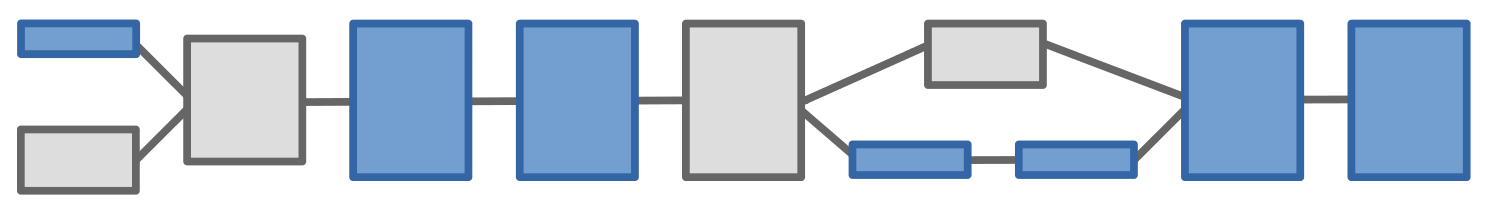
\includegraphics[width=0.6\linewidth]{figures/dag_ABCDE.png}
  \caption{An example of a DAG representing clusters of SSEs. 
  The height of each rectangle shows the number of SSEs in the cluster.
  The color shows the cluster type (gray = helix, blue = strand).
  The direction of the edges is implicit (left to right).
  The egdes that can be inferred from transitivity are not shown 
  (i.e. we show only the transitive reduction). }
  \label{fig:dag_example}
\end{figure}

The merging step follows the guide tree. First, each guide tree leaf is
populated with the DAG of SSEs of its respective domain (in the leaves the DAG is always a path). 
In each internal node, the DAGs from the two children nodes are matched together and merged. 
The root then contains the consensus SSEs of the whole family (see Figure \ref{fig:dag_merging}). 

\begin{figure}[h!]
  \centering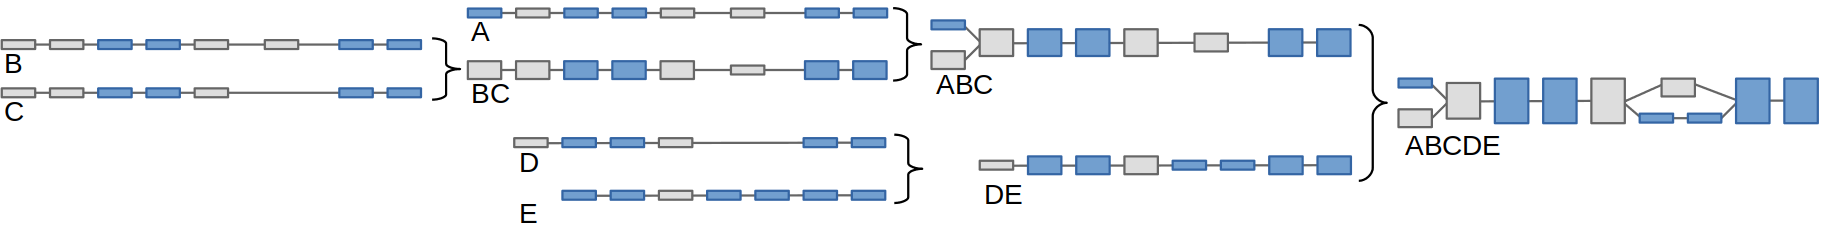
\includegraphics[width=\linewidth]{figures/dag_merging.png}
  \caption{The process of merging 5 DAGs based on the guide tree from Figure \ref{fig:guide_tree}.}
  \label{fig:dag_merging}
\end{figure}

The matching and merging of two SSE graphs is in principle similar to matching (aligning)
and merging of two weighted structures. The best matching is also found
by dynamic programming. However, it is more complicated here, because 1)
clusters of different type cannot be matched (this can cause the
branching in the resulting DAG), and 2) the dynamic programming
algorithm is not as straightforward for matching DAGs as it is for
matching sequences.

The β-connectivity is not directly considered in the merging algorithm 
(though it is included in the distance function for DAG matching).
Therefore it is necessary to determine the β-connectivity of the resulting clusters 
based on the β-connectivity of the original SSEs.

A β-ladder \(UVo\) (connecting strand clusters \(U\) and \(V\) with orientation \(o\) (parallel/antiparallel)) 
is included in the resulting consensus if

\[  \frac { n_{UVo} } { \min{\{n_U, n_V\}} } \geq 0.5  \]

where \(n_U\) is the number of strands in cluster \(U\), 
\(n_V\) is the number of strands in cluster \(V\),
and \(n_{UVo}\) is the number of ladders connecting a strand in \(U\) to a strand in \(V\)
with orientation \(o\) (see Figure \ref{fig:dag_ladders}).

\begin{figure}[h!]
  \centering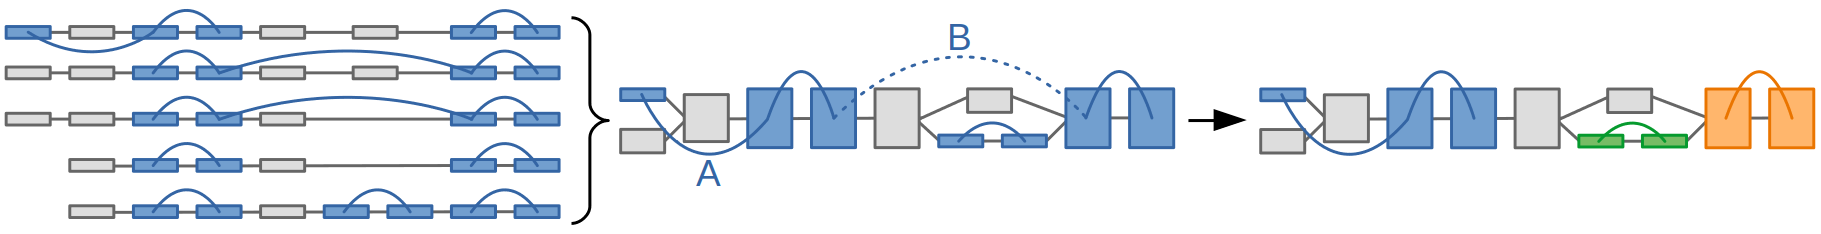
\includegraphics[width=\linewidth]{figures/dag_ladders.png}
  \caption{Merging β-ladders from 5 domains. 
  Lower arcs show parallel, upper arcs antiparallel ladders.
  Ladder A is included because \( n_{UVo} / \min{\{n_U, n_V\}} = 1 / \min{\{1, 5\}} = 1 \geq 0.5\).
  Ladder B is not included because \( n_{UVo} / \min{\{n_U, n_V\}} = 2 / \min{\{5, 5\}} = 0.4 < 0.5\).
  The last column shows the separation of the consensus strands into sheets (connected components).}
  \label{fig:dag_ladders}
\end{figure}



%%%%%%%%%%%%%%%%%%%%%%%%%%%%%%%%%%%%%%%%%%%%%%%%%%%%%%%%%%%%%%%%%%%%%%%%%%%%
\subsection{Annotation}

This is an optional step, in which the generated SSE consensus is used
as annotation template for SecStrAnnotator and all family members are
annotated. Before the annotation, the SSEs with low occurrence
(\textless{} 5\%) are removed, which dramatically reduces the running
time of SecStrAnnotator. Options for SecStrAnnotator:
\code{-\/-ssa\ file} ~\code{-\/-align\ none}
~\code{-\/-metrictype~3} ~\code{-\/-fallback\ 30}
~\code{-\/-unannotated}.



%%%%%%%%%%%%%%%%%%%%%%%%%%%%%%%%%%%%%%%%%%%%%%%%%%%%%%%%%%%%%%%%%%%%%%%%%%%%
\subsection{Visualization}

The generated SSE consensus is visualized by several SVG diagrams with
different settings and \path{diagram.json} file is produced, which
will be used for interactive visualization by OverProt Viewer. A PyMOL
session (.pse) is created, with the structure consensus from MAPSCI
(shown as ribbon) and the SSE consensus (shown as cylinders and arrows).
The width of each cylinder/arrow shows to the occurrence of the corresponding helix/strand.
A PNG image is also rendered from the session. 
A session with all domains and their SSEs is
generated if \code{{[}visualization{]}create\_multi\_session} is
\code{True} (very slow, not recommended for larger families).



%%%%%%%%%%%%%%%%%%%%%%%%%%%%%%%%%%%%%%%%%%%%%%%%%%%%%%%%%%%%%%%%%%%%%%%%%%%%
\subsection{Execution}

OverProt Core is implemented mostly in Python 
and designed to run in the Linux environment (tested on Ubuntu 20.04).
On the other operating systems, it can be run in Docker.
Before the first execution, the dependencies must be installed:

\begin{codeblock}
  sh install.sh --clean
\end{codeblock}

All steps of the algorithm are combined in \path{overprot.py}. 
It is run in a Python virtual environment. 
The arguments are the CATH family ID and the output directory.

\begin{codeblock}
  . venv/bin/activate
  python overprot.py --help
  python overprot.py 1.10.630.10 data/cyp/
\end{codeblock}

Multiple families can be processed in parallel using \path{overprot_multifamily.py}. 
The arguments are the family list and the output directory.

\begin{codeblock}
  . venv/bin/activate
  python overprot_multifamily.py --help
  python overprot_multifamily.py data/families.txt data/multifamily/
\end{codeblock}


%%%%%%%%%%%%%%%%%%%%%%%%%%%%%%%%%%%%%%%%%%%%%%%%%%%%%%%%%%%%%%%%%%%%%%%%%%%%%%
%%%%%%%%%%%%%%%%%%%%%%%%%%%%%%%%%%%%%%%%%%%%%%%%%%%%%%%%%%%%%%%%%%%%%%%%%%%%%%
\section{Interactive visualization by OverProt Viewer}

\textbf{OverProt Viewer} is a web component for interactive
visualization of the SSE consensus. Its input is the preprocessed
\path{diagram.json} file. It is implemented in TypeScript with D3.js.



%%%%%%%%%%%%%%%%%%%%%%%%%%%%%%%%%%%%%%%%%%%%%%%%%%%%%%%%%%%%%%%%%%%%%%%%%%%%%%
%%%%%%%%%%%%%%%%%%%%%%%%%%%%%%%%%%%%%%%%%%%%%%%%%%%%%%%%%%%%%%%%%%%%%%%%%%%%%%
\section{Data computation for OverProt Server}

\textbf{OverProt Server} serves precomputed SSE consensuses (database)
and runs the OverProt Core algorithm for user-defined sets of domains
(jobs).

The database is constructed in this way:

\begin{itemize}
\item
  Retrieve the current list of families from CATH
  (\path{ftp://orengoftp.biochem.ucl.ac.uk/cath/releases/latest-release/cath-classification-data/cath-domain-list.txt}).
  (This file also contains the domain definitions, but they are in an
  incompatible numbering scheme (\emph{auth*}), therefore they are not
  used). This is currently 6631 families, out of which 64 are empty
  families (December 2021).
\item
  Retrieve the domain lists for each family, including chains and
  residue ranges, from PDBe API
  (\path{https://www.ebi.ac.uk/pdbe/api/mappings/{family_id}}). This is
  currently over 470k domains (December 2021).
\item
  Remove duplicates (i.e.~multiple domains from the same PDB entry).
  This is currently over 200k domains (December 2021).
\item
  Apply the OverProt Core algorithm to each family.
\end{itemize}

The whole process is realized by:

\begin{codeblock}
    python  overprot_multifamily.py  --download_family_list_by_size
    --config working_scripts/overprot-config-overprotserverdb.ini
    --collect  xxx  all  $UPDATE_DIRECTORY                                                     $
\end{codeblock}

The database is updated weekly.



%%%%%%%%%%%%%%%%%%%%%%%%%%%%%%%%%%%%%%%%%%%%%%%%%%%%%%%%%%%%%%%%%%%%%%%%%%%%%%
%%%%%%%%%%%%%%%%%%%%%%%%%%%%%%%%%%%%%%%%%%%%%%%%%%%%%%%%%%%%%%%%%%%%%%%%%%%%%%
\section{Appendix}



%%%%%%%%%%%%%%%%%%%%%%%%%%%%%%%%%%%%%%%%%%%%%%%%%%%%%%%%%%%%%%%%%%%%%%%%%%%%
\subsection{Computation of distance function for two weighted structures}

A weighted structure \(A\) is a tuple
\( (n^A, \mathbf{R}^A, \mathbf{W}^A, k^A) \) where \(n^A\) is the length
of the weighted structure (number of points), \(\mathbf{R}^A\) is the
matrix of their coordinates (\(n^A \times 3\)), \(\mathbf{W}^A\) is the
vector of their relative weights \(\in (0,1]\), and \(k^A\) is the
absolute weight of \(A\). Example of a weighted structure:

\[
  n^A = 4 \quad
  \mathbf{R}^A = \begin{bmatrix}-1.1&-2.9&0.1&0.4\\0.0&1.1&0.9&-2.7\\5.2&2.1&0.0&0.8\end{bmatrix} \quad
  \mathbf{W}^A = \begin{bmatrix}1&0.5&0.8&1\end{bmatrix} \quad
  k^A = 10
\]

\(\mathbf{r}^A_i\) and \(w^A_i\) will refer to \(i\)-th column of
\(\mathbf{R}^A\) and \(\mathbf{W}^A\).

\TODO{nice format (matrices and vectors in bold)}

A protein domain can be converted into a weighted structure as follows:
\(n\) is the number of residues, \(\mathbf{r}^A_i\) are the coordinates of the
C-alpha atom of \(i\)-th residue, \(w^A_i\) is 1, and \(k^A\) is 1.

The distance function \(d\) is defined for two weighted points:

\[
  d \left( (\mathbf{r}^A_i, w^A_i), (\mathbf{r}^B_j, w^B_j) \right) 
  = \left( 1 - e^{-\lVert \mathbf{r}^A_i-\mathbf{r}^B_j \rVert / R_0} \right) \cdot \min\{ w^A_i, w^B_j \} + \frac{1}{2} \lvert w^A_i-w^B_j \rvert
\]

In case that one of the weighted points is undefined (\(\bot\)), \(d\)
is still defined:

\[
  d \left( (\mathbf{r}^A_i, w^A_i), \bot \right) = \frac{1}{2} w^A_i \qquad 
  d \left( \bot, (\mathbf{r}^B_j, w^B_j) \right) = \frac{1}{2} w^B_j
\]

(Note: Distance \(d\) is not the Euclidean distance of the two points.
\(d \in [0,1)\).)

An alignment of two weighted structures \(A\), \(B\) is a sequence of
pairs \([(p_1, q_1), (p_2, q_2), ..., (p_n, q_n)]\) (for better reading
written as a matrix
\(\begin{bmatrix}p_1&p_2&...&p_n\\q_1&q_2&...&q_n\end{bmatrix}\)), where
\(p_i\) and \(q_i\) are indices of the points of \(A\) and \(B\).
Indices must be increasing and must include each index exactly once for
both \(A\) and \(B\). Value \(\bot\) means that a particular point was
not matched. Example of a valid alignment for \(n^A = 4, n^B = 5\):

\[\begin{bmatrix}1&2&3&4&\bot&\bot\\1&\bot&2&3&4&5\end{bmatrix}\]

The distance function \(D\) for two weighted structures \(A\) and \(B\) with a given alignment \(M\) is defined:

\[  D(A, B, M) = \sum\limits_{(p, q) \in M}{d \left( (\mathbf{r}^A_{p}, w^A_{p}), (\mathbf{r}^B_{q}, w^B_{q}) \right)}  \]

The distance function \(D^*\) of two weighted structures \(A\) and \(B\) is then:

\[  D^*(A, B) = D(A, B, M^*)  \]

where \(M^*\) is the best alignment of \(A\) and \(B\), i.e. the alignment which minimizes \(D(A, B, M^*)\).

The best alignment is found by dynamic programming (this is basically
the Needleman-Wunsch algorithm {[}cite{]}). For this, the distance
function \(d\) is converted into a score function \(s\):

\[
  s \left( (\mathbf{r}^A_i, w^A_i), (\mathbf{r}^B_j, w^B_j) \right) 
  = \frac{1}{2} w^A_i + \frac{1}{2} w^B_j - d \left( (\mathbf{r}^A_i, w^A_i), (\mathbf{r}^B_j, w^B_j) \right)
\]

\[
  s \left( (\mathbf{r}^A_i, w^A_i), \bot \right) = 0 \qquad 
  s \left( \bot, (\mathbf{r}^B_j, w^B_j) \right) = 0
\]

Similarly, \(D\) is converted into \(S\):

\[
  S(A, B, M) 
  = \sum\limits_{(p, q) \in M}{s \left( (\mathbf{r}^A_{p}, w^A_{p}), (\mathbf{r}^B_{q}, w^B_{q}) \right)}
  = \sum\limits_{i=1}^{n^A}{w^A_i} + \sum\limits_{j=1}^{n^B}{w^B_j} - D(A, B, M)
\]

From this equation it can be seen, that maximizing \(S\) by dynamic
programming also minimizes \(D\).

A useful property of the distance function \(D^*\) is that it is a
metric (i.e.~\(D^*(A,A) = 0\), \(D^*(A,B) = D^*(B,A)\), and
\(D^*(A,B) + D^*(B,C) \geq D^*(A,C)\) for any weighted structures
\(A, B, C\)).



%%%%%%%%%%%%%%%%%%%%%%%%%%%%%%%%%%%%%%%%%%%%%%%%%%%%%%%%%%%%%%%%%%%%%%%%%%%%
\subsection{Merging two weighted structures}

Having two weighted structures \(A, B\) and their best alignment
\(M^*(A, B) = [(p_1, q_1), ..., (p_n, q_n)]\), we can define operation
\(merge\) as follows:

\[  merge(A, B) = C = (n^C, \mathbf{R}^C, \mathbf{W}^C, k^C)  \]

\[  n^C = n  \]

\[  \mathbf{r}^C_i = \frac {\mathbf{r}^A_{p_i} w^A_{p_i} k^A + \mathbf{r}^B_{q_i} w^B_{q_i} k^B} {w^A_{p_i} k^A + w^B_{q_i} k^B}  \]

\[  w^C_i = w^A_{p_i} k^A + w^B_{q_i} k^B  \]

\[  k^C = k^A + k^B  \]

(If \(p_i=\bot\), the values can be calculated by setting
\(w^A_{p_i} = 0\), thus simplifying to
\(\mathbf{r}^C_i = \mathbf{r}^B_{q_i}, w^C_i = w^B_{q_i}\). Similarly for \(q_i=\bot\).)

Remark: When finding the two nearest items in the work set, it is not
necessary to calculate the distance \(D^*\) for every pair of items --
there are specialized data structures that can significantly decrease
the number of distance calculations. We use a non-standard structure
NN-tree (nearest neighbour tree). In some larger protein families this
can reduce the number of distance computations to roughly 20\%. 
(Standard structures like VP-tree, GH-tree, GNAT, M-tree etc. 
(\TODO{name what I tried}) either miss some of
the necessary operations (insert, delete) or perform worse than NN-tree
for this particular application.)




%%%%%%%%%%%%%%%%%%%%%%%%%%%%%%%%%%%%%%%%%%%%%%%%%%%%%%%%%%%%%%%%%%%%%%%%%%%%%%
%%%%%%%%%%%%%%%%%%%%%%%%%%%%%%%%%%%%%%%%%%%%%%%%%%%%%%%%%%%%%%%%%%%%%%%%%%%%%%
\section{References}


\end{document}